\section{Introduction to GIRAF}\label{sec:giraf-intro}
This section introduces the structure of GIRAF and how its way of communicating to people suffering from ASD, pictograms.
Firstly the current applications will be shortly introduced.
Then the concept of a pictogram will be introduced and their use in GIRAF.
If the reader is already familiar with these concepts then the rest of this section can be skipped.

\subsection{Contents of the GIRAF Application Suite}
This section will present the GIRAF application suite, which applications it contains and what they do.
Currently 11 applications are published on the Google Play Store under the developer name \textit{GIRAF Autism Apps}\footnote{\url{https://play.google.com/store/apps/developer?id=GIRAF+Autism+Apps}}.
Some apps are required for GIRAF to run, while others are optional.
The fact that some are required has to due to with the applications having originally been developed by different groups as individual small applications, rather than one big collaborative applicaiton, this includes the launcher and administrative tools.
However it is recommended that all the applications is downloaded before use, in order to see the full picture of what the application suite offers.
The following section will introduce the different applications of GIRAF, and give a brief explanation of their functionality.
\begin{description}
	\item[GIRAF (Main Launcher)]\hfill \\
	The GIRAF Launcher is meant to replace the default launcher of the device and is used to launch the applications of the GIRAF Application Suite, but could also be used to launch other third party applications.
	It has a home screen like any android OS has, which is where the applications can be launched from.
	Additionally the options menu and administration panel is opened from here.
	\item[Administration Tool]\hfill \\
	The Administration Tool is primarily used by guardians to configure which applications each citizen can utilise.
	\item[Sequence] \hfill \\
	Sequence (also known as \enquote{Sekvens} in Danish) is a tool used to create sequences of pictograms for use in other parts of the application.
	These pictograms, which is a pictorial symbol of a phrase or word, is what the citizens sometimes communicate by, and this is also what helps them create these rigid plans, e.g. for going to the bathroom.
	\item[Week Schedule] \hfill \\
	Week Schedule (also know as \enquote{Ugeplan} in Danish) uses pictograms to display a schedule for each day of the week one week at a time.
	\item[Pictosearch] \hfill \\
	Pictosearch is used to search through the pictograms such that they can be used for other applications.
	\item[Pictoreader] \hfill \\
	The Pictoreader can display and read out-loud a series of pictograms.
	\item[Category Manager] \hfill \\
	The Category Manager (also known as \enquote{Kategoriværktøjet} in Danish) is used to manage categories of pictograms for use in other applications most notably the Category Game.
	It is also used to more easily be able to find certain pictograms, without having to use Pictosearch.
	\item[Category Game] \hfill \\
	The Category Game (also known as \enquote{Kategorispillet} in Danish) is a game that asks the player to group up different pictograms into categories either predefined or defined in the Category Manager.
	The game itself consists of a train which must drop off the pictograms at different stations according to their grouping.
	\item[Timer] \hfill \\
	The timer (also known as \enquote{Tidstager} in Danish) is an application which can limit the amount of time another application is allowed to be active for.
	This is often useful in combination with the Week Schedule, which can feature elements like, e.g., 10 minutes of playing the Category Game, or how long a third party application, e.g. a video game, could be open for.
	\item[Life Story] \hfill \\
	Life Story (also known as \enquote{Livshistorier} in Danish) is similar to the Sequence application but is used to remember what actions were taken by a citizen throughout the day, or as a way of communicating since some citizens have a lot of trouble with their verbal communication.
	It is meant to give the citizens a way to communicate with other people other than verbally.
	They can create a set of pictograms showing what they did in the weekends and then show others these stories.
	\item[Voice Game] \hfill \\
	Voice Game (also known as \enquote{Stemmespillet} in Danish) is a game in which the purpose is to control a car, either avoiding obstacles or gathering stars, using only your voice.
	This is supposed to help the citizens learn to control the volume of their voice, as some has troubles with either speaking too loudly too silently.
	\item[Web Admin] \hfill \\
	There is also a web view for GIRAF which is where the creation of new users is done.
	It is not very developed, but the vision is that it will be able to create week schedules for citizens as well so that the guardians can choose to use a computer rather than a tablet to do their work.

\end{description}

\subsection{Pictograms}
Pictograms are used in many places throughout the GIRAF project.
A pictogram is an image which resembles an action or an object.
Pictograms are used in place of text since many of the citizens using the GIRAF project is not able to read.
Two examples of pictograms are shown in~\myref{fig:pictograms}.

% https://en.wikibooks.org/wiki/LaTeX/Floats,_Figures_and_Captions#Subfloats
\begin{figure}[H]
    \centering
    \begin{subfigure}[b]{0.2\textwidth}
    	\fbox{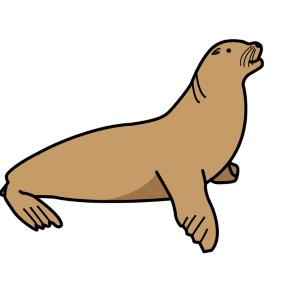
\includegraphics[width=\dimexpr\textwidth-2\fboxsep-2\fboxrule\relax]{figures/pictograms/pictogramsealion.png}}
        \caption{Sealion}
        \label{fig:sealion}
    \end{subfigure}
    \qquad
    \begin{subfigure}[b]{0.2\textwidth}
		\fbox{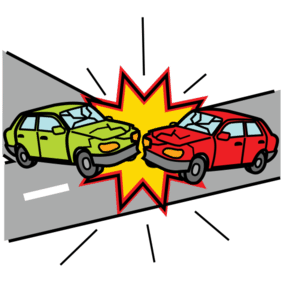
\includegraphics[width=\dimexpr\textwidth-2\fboxsep-2\fboxrule\relax]{figures/pictograms/pictogramtrafficcolision.png}}
        \caption{Traffic Collision}
        \label{fig:traffic_collision}
    \end{subfigure}
    \caption{Examples pictograms.}\label{fig:pictograms}
\end{figure}

Pictograms will often appear with an icon indicating something about them, these icons are called emblems.
This is to indicate what actions are available, pressing the pictogram will perform an action, such as a trash bin indicating that a deletion will happen when tapping the pictogram with the bin.
Two examples of this is shown in~\myref{fig:pictograms_with_indicators}

\begin{figure}[H]
    \centering
    \begin{subfigure}[b]{0.2\textwidth}
    	\fbox{
\includegraphics[width=\dimexpr\textwidth-2\fboxsep-2\fboxrule\relax]{figures/pictograms/pictogramsealion_with_indicator.png}}
        \caption{Sea lion with wrench}
        \label{fig:sealion-with-wrench}
    \end{subfigure}
    \qquad
    \begin{subfigure}[b]{0.2\textwidth}
		\fbox{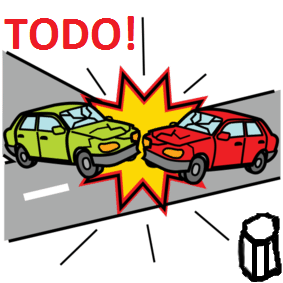
\includegraphics[width=\dimexpr\textwidth-2\fboxsep-2\fboxrule\relax]{figures/pictograms/pictogramtrafficcolisionn_with_indicator.png}}
        \caption{Traffic Collision with trash bin}
        \label{fig:trafficcollision-with-wrench}
    \end{subfigure}
    \caption{Examples pictograms with emblems.}\label{fig:pictograms_with_indicators}
\end{figure}

